% Chapter X

\chapter{Validation of the Heat Flux Partitioning Model} % Chapter title

\label{ch:HFP_validation} % For referencing the chapter elsewhere, use \autoref{ch:name} 

%----------------------------------------------------------------------------------------

In this Chapter, we want to assess the validity of the new Heat Flux Partitioning formulation proposed in Chapter \ref{chap:HFP_closures}. To do so, we will conduct two different validations:

\begin{itemize}
\setlength{\itemsep}{8pt}
\item The first part will be dedicated to validation on a single experimental subcooled boiling case at 10.5 bar from Kossolapov \cite{kossolapov_experimental_2021} for which numerous physical parameters have been measured. This will ensure that the proposed mathematical formulation and the closure laws propose an acceptable physical modeling of the boiling parameters.

\item The second part will consist on wall temperature predictions for vertical subcooled flow boiling of water in various conditions, including pressure. Experimental database from Jens \& Lottes \cite{jens_analysis_1951}, Kennel \cite{kennel_local_1949} and Kossolapov \cite{kossolapov_experimental_2021}. Comparison with other HFP models from Kurul \& Podowski, Basu and Kommajosyula will be performed.
\end{itemize}


\section{Detailed Comparison and Assessment of the Heat Flux Partitioning}

In this section, we compare our results to those obtaines by Kossolapov \cite{kossolapov_experimental_2021} in vertical subcooled flow boiling. At a pressure of 10.5 bar, he realized measurements of many relevant parameters regarding the Heat Flux Partitioning:

\begin{itemize}
\item Active nucleation site density $N_{sit,a}$ ;
\item Bubble nucleation frequency $f$ ;
\item Bubble wait time $t_{w}$ ;
\item Transient heat transfer (quenching) time $t_{q}$ ;
\item Average bubble growth time $t_{g}$ ;
\item Average area visited by a bubble $A_{q,1b}$ ;
\item Proportion of the heater area impacted by bubbles $A_{b,tot}$
\item Liquid single-phase heat flux proportion $\dfrac{\phi_{c,L}}{\phi_{w}}$ ;
\item Quenching heat flux proportion $\dfrac{\phi_{q}}{\phi_{w}}$ ;
\item Wall superheat $\Delta T_{w}$.
\end{itemize}

The only lacking parameters to conduct a full evaluation of the model would be the average bubble departure diameter $R_{d}$, sliding length $l_{sl}$ and lift-off diameter / coalescence diameter.

The values provided by Kossolapov are an average conducted over all the observed nucleation events during the time of the experiment. Such data are representative of what we want to achieve using a HFP model since we represent average values of the boiling parameters for the considered boiling surface.

\npar

All those variables were measured for a subcooling $\Delta T_{L} = 10\degC$ at three different liquid mass fluxes $G_{L} = 500$, $1000$ and $2000~\debm$. 

\npar

We present the results obtained by comparison with the case at $G_{L} = 2000 \debm$ for each variable. The simulations using the HFP model were conducted using a contact angle $\theta = 80 \degree$ (usual contact angle for water and ITO \cite{kossolapov_experimental_2021}), an hysteresis $\dtheta = 2 \degree$ and a growth constant $K=1.5$

 
\subsection{Active Nucleation Site Density}

On Figure \ref{fig:fullkoss_nsit}, we compare the values obtained for the active nucleation site density. The Li \etal correlation used in the model (Eq. \ref{eq:nsit_li}) propose a reasonable prediction of the measured values of $N_{sit,a}$ with an underestimation of less than a decade. The correlation correctly reproduce the experimental trend where we observe a sort of saturation in the nucleation site density for higher wall superheat.

\npar

To better match the asymptotic value of the experiment, we correct the Li \etal correlation for this case by a factor $\Delta T_{w}^{3-0.6\Delta T_{w}^{0.5}}$ which better fits the measurements for $\Delta T_{w}>10$~K but yields a small overestimation before.


\begin{figure}[!h]
\subfloat[$N_{sit,a}$ predictions by Li \etal correlation]{
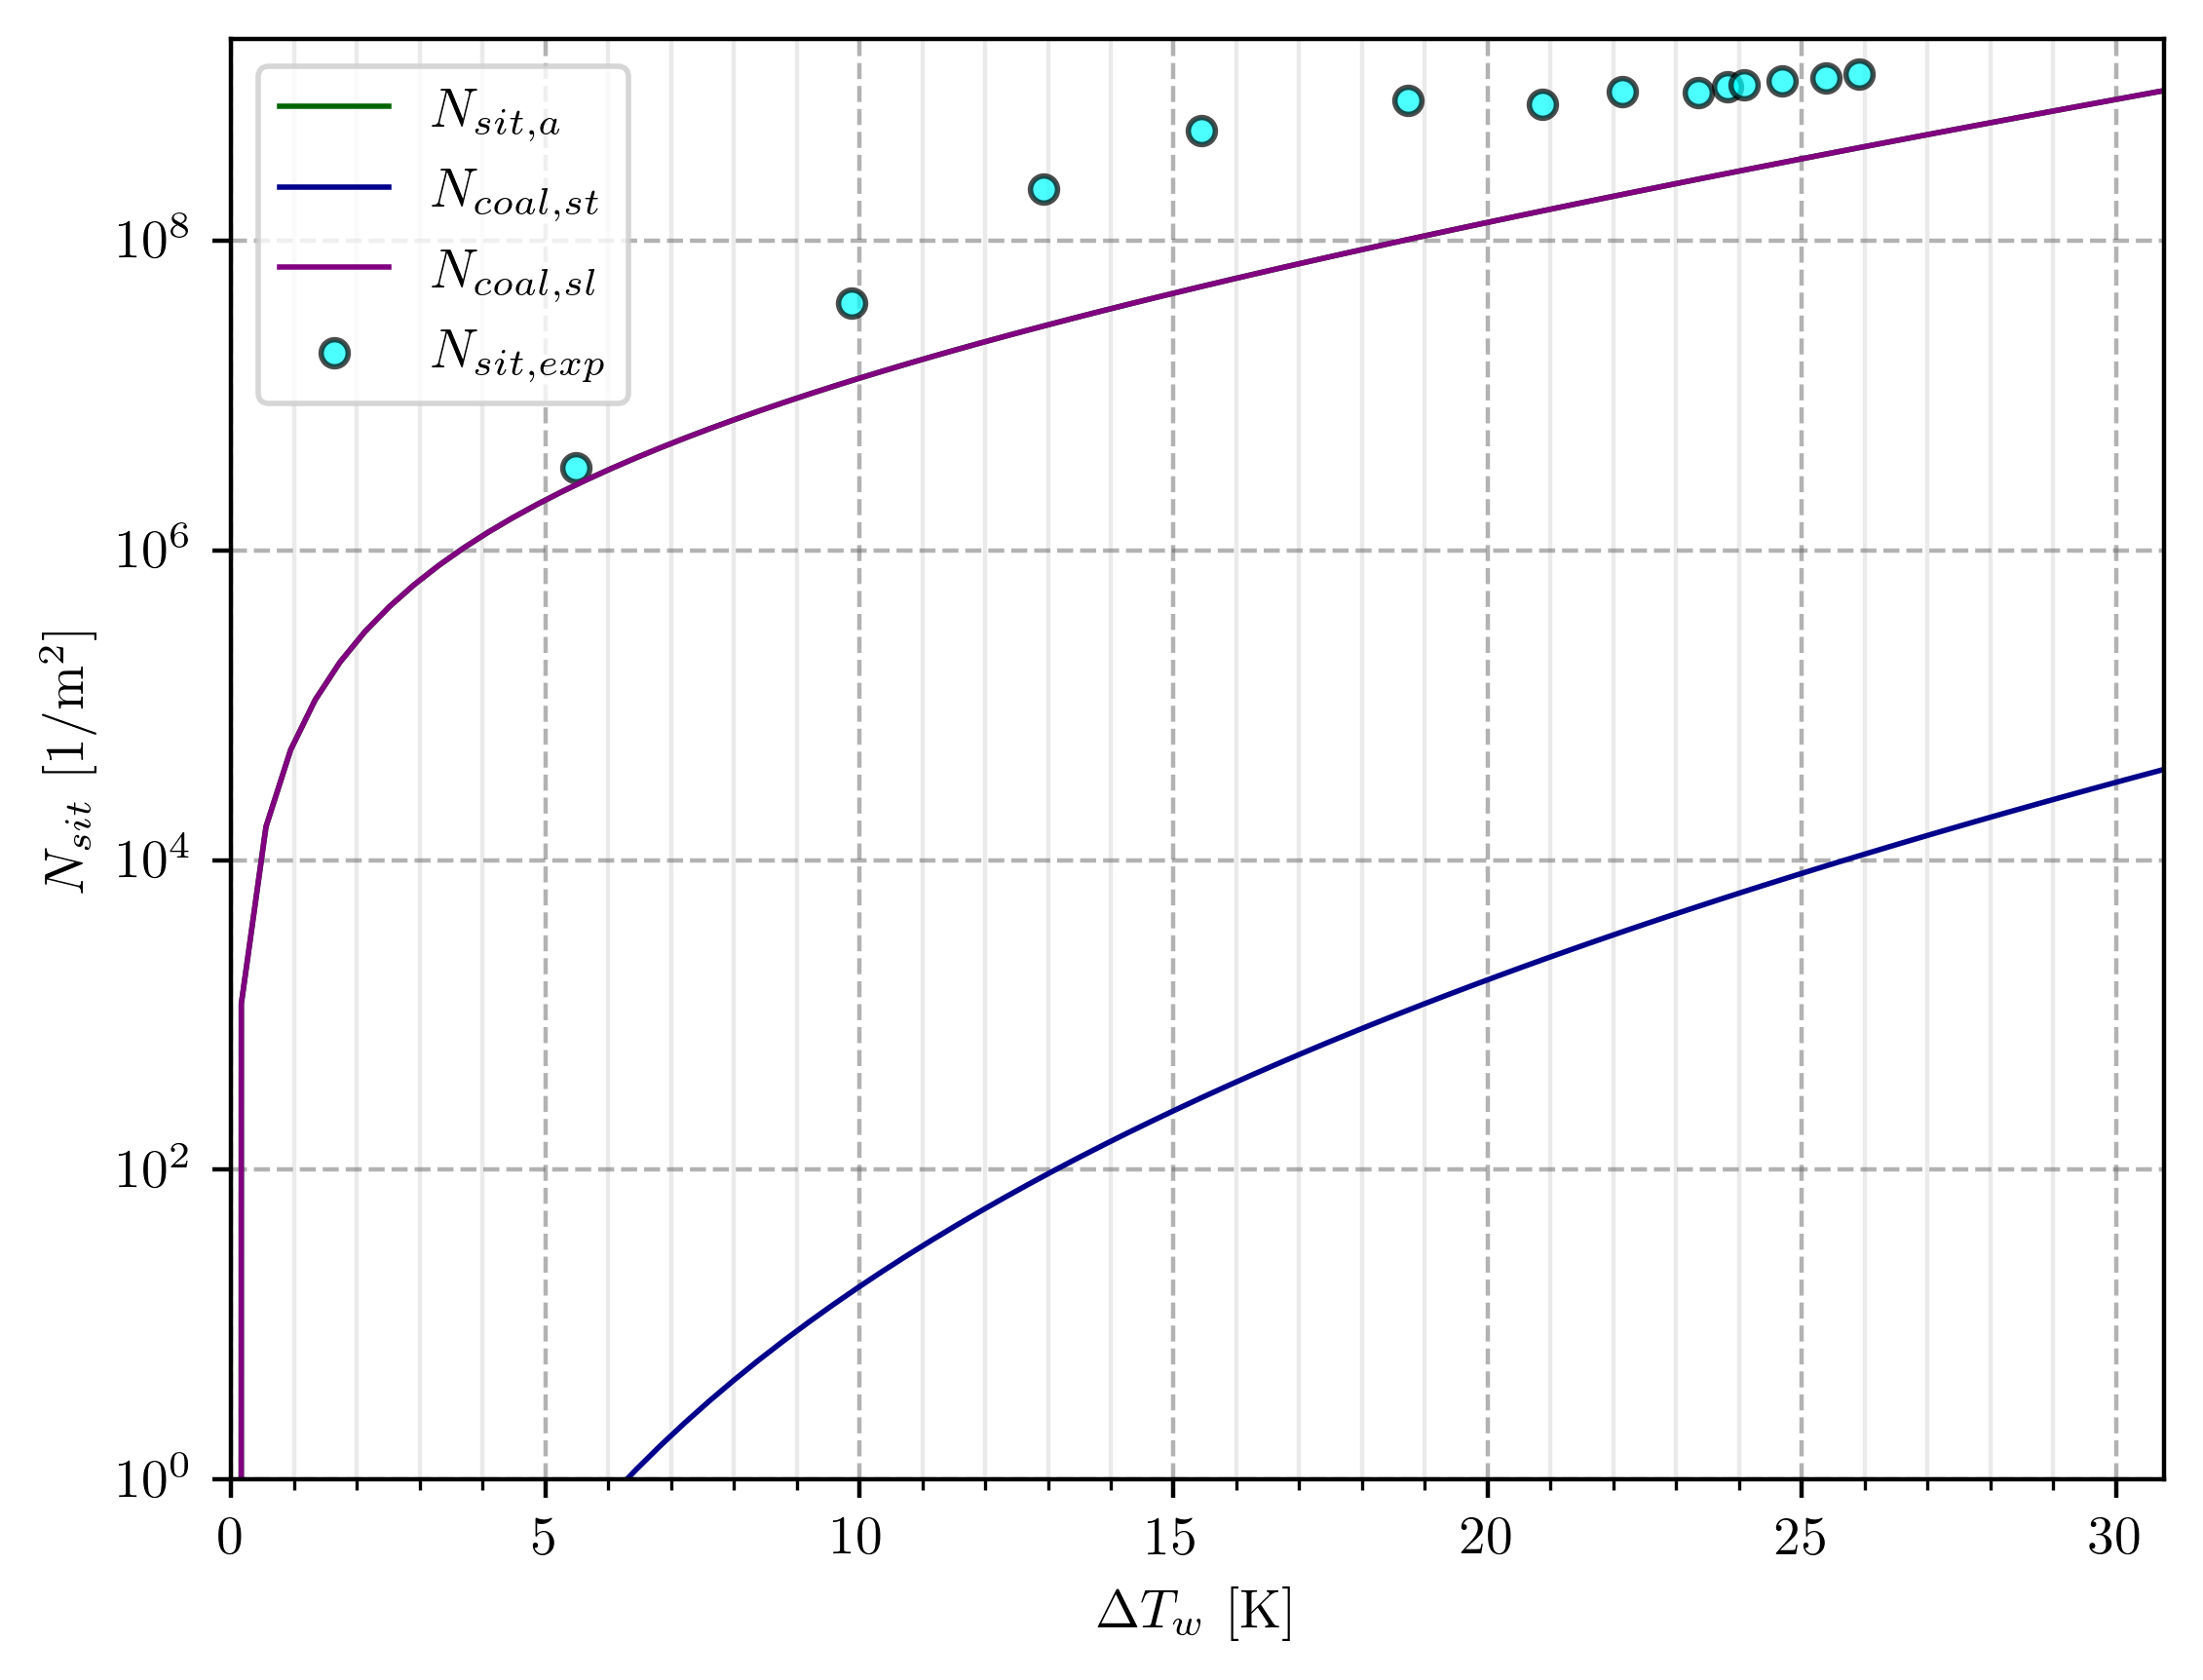
\includegraphics[width=0.5\linewidth]{img/HFP/fullcomp_Koss/sites_G2000_nocorr.png}
}
\subfloat[$N_{sit,a}$ predictions with corrected Li \etal correlation]{
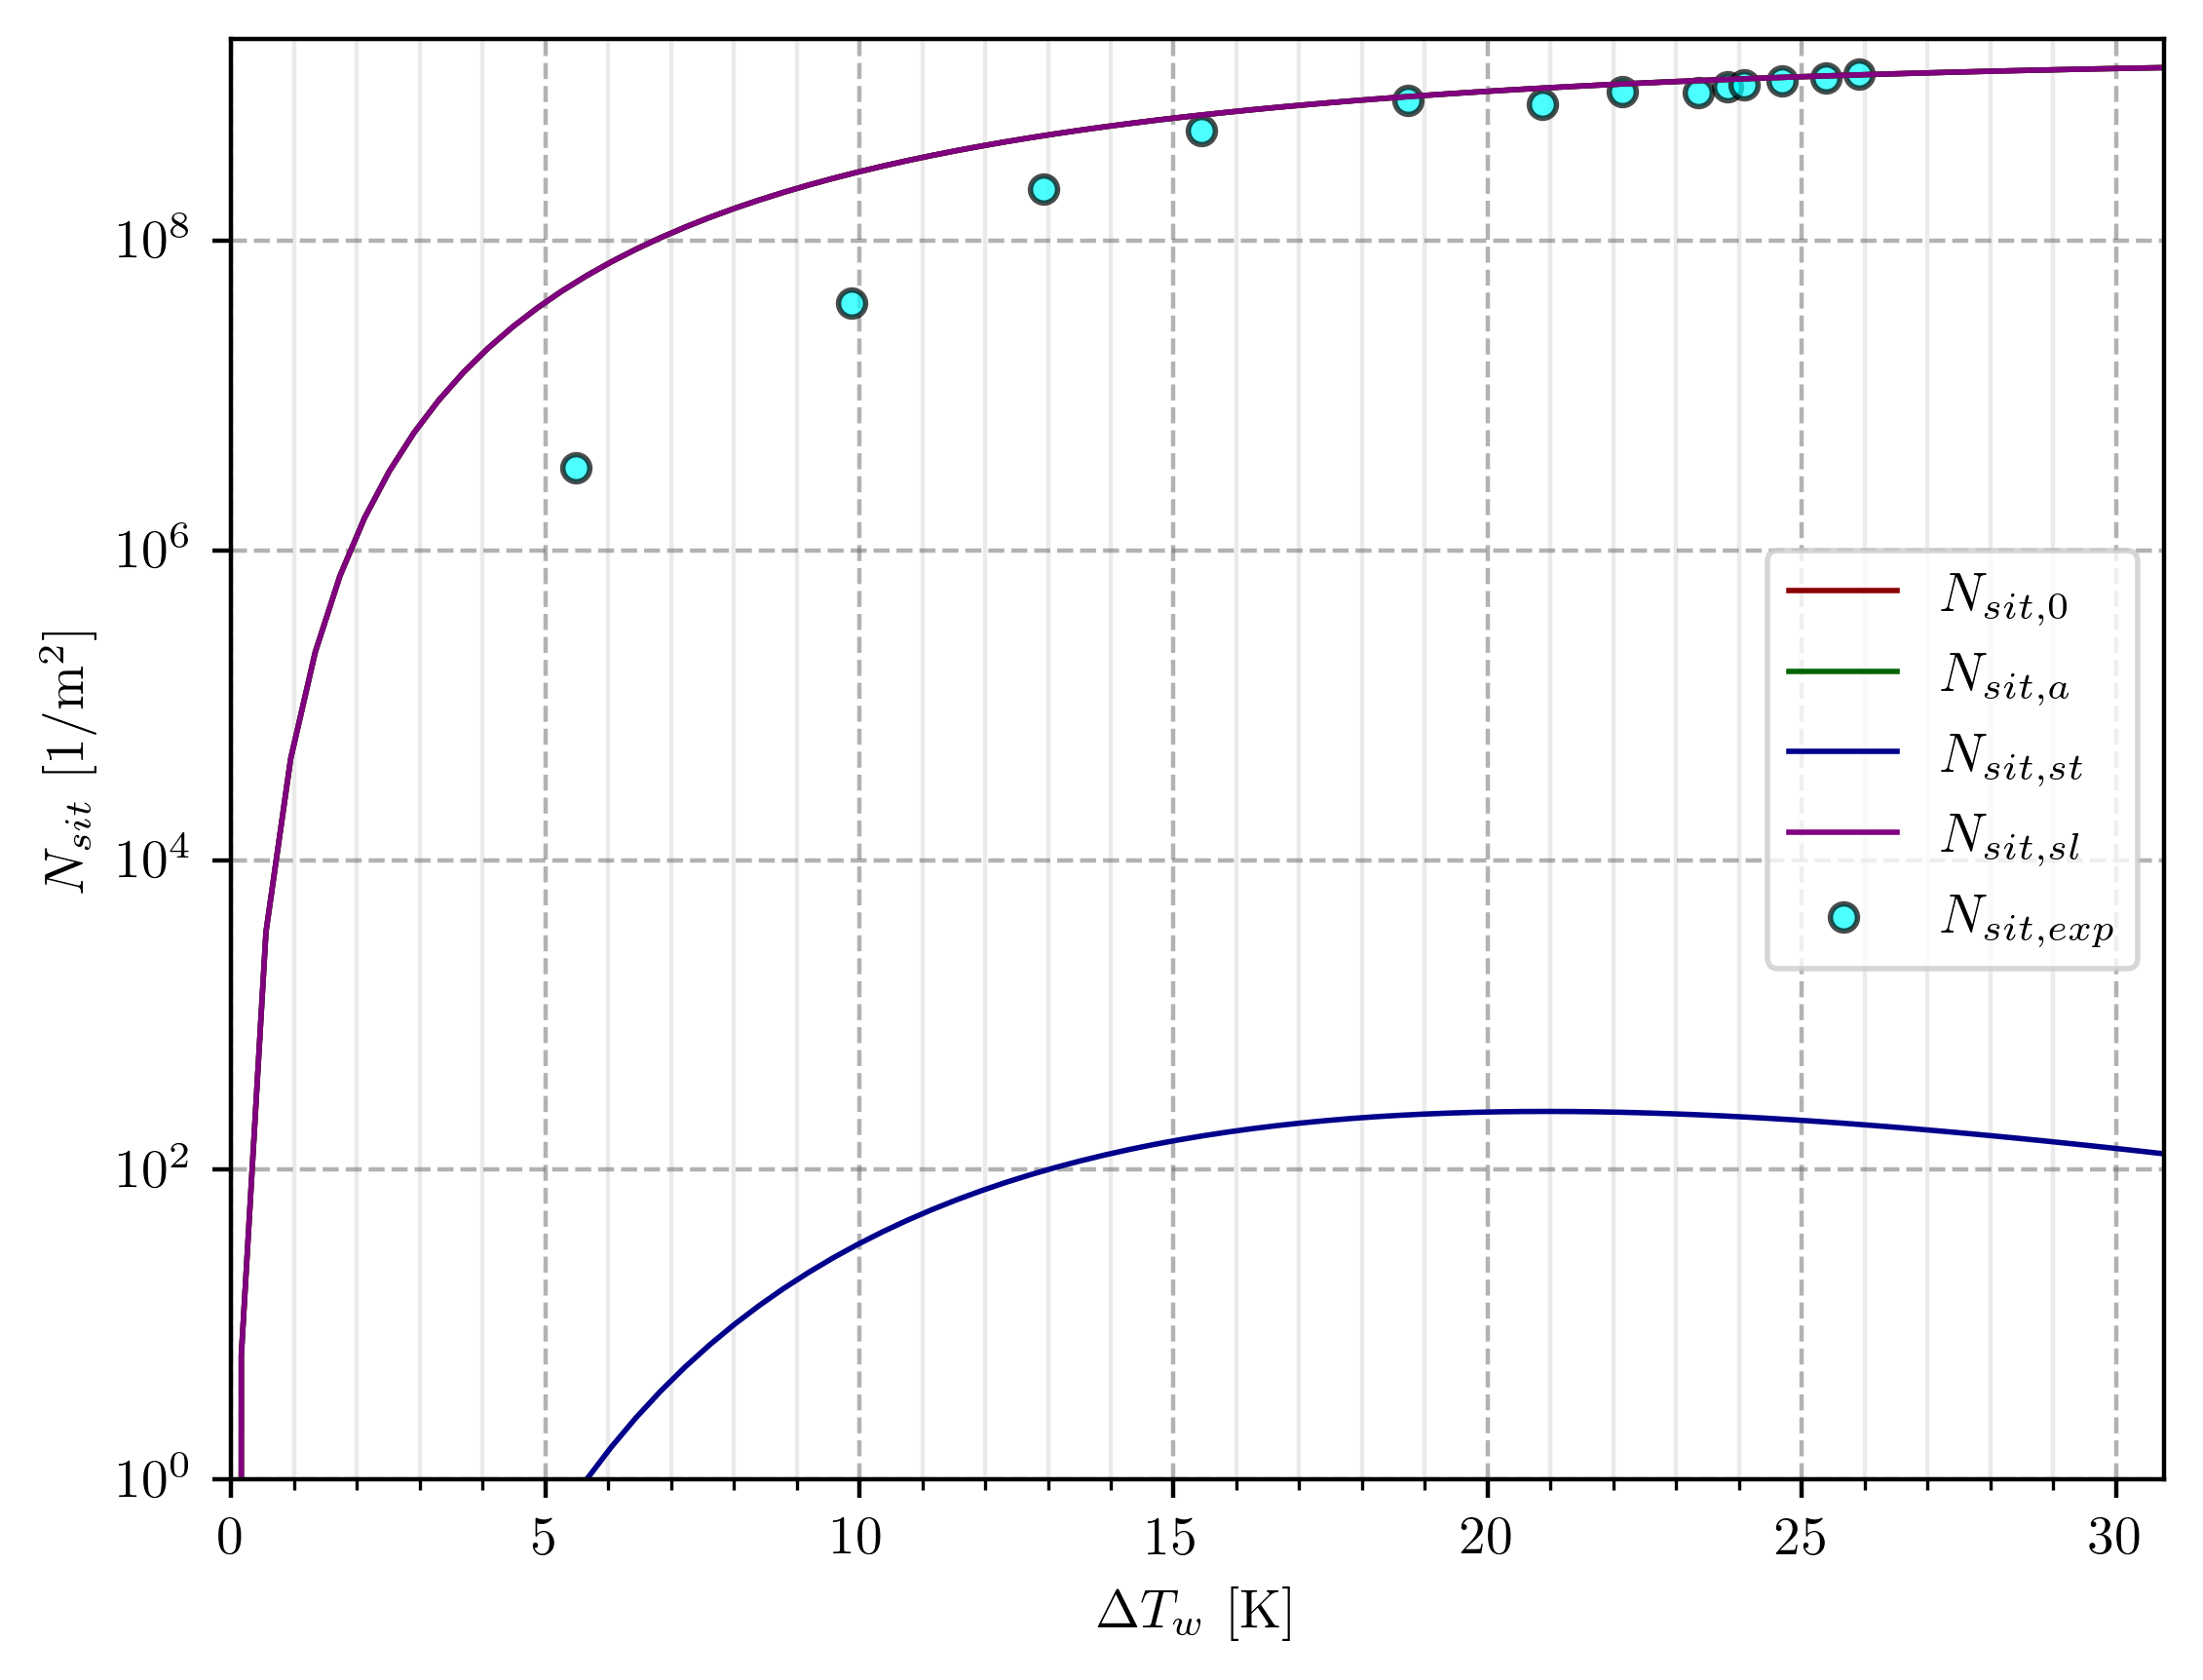
\includegraphics[width=0.5\linewidth]{img/HFP/fullcomp_Koss/sites_G2000.png}
}
\caption{Comparison of active nucleation site density with and without a correction for Li \etal formulation.}
\label{fig:fullkoss_nsit}
\end{figure}



\subsection{Wait Time, Growth Time, Quenching Time and Nucleation Frequency}

Figure \ref{fig:fullkoss_times} compares the different times involved in the boiling physics and the bubble nucleation frequency. As seen in Sec \ref{sec:wait_time}, the wait time is quite fairly reproduced along with the nucleation frequency. Actually, the bubble departure is nearly instantaneous and the nucleation cycle is mainly composed of the wait period, which means a good estimation of $t_{w}$ leads to a reasonable estimation of $f$ for this case.

\npar

The average bubble growth time is overestimated by nearly a decade for low superheat and is better predicted for larger superheat. Its evolution seem coherent with a decrease up to 15\ K and a stabilization afterwards. However, the experimental measurements show an increase in the growth time for large superheat which could be associated to bubble diameter increase with the wall Jakob number as previously observed in Section \ref{sec:liftoff}.



\begin{figure}[!h]
\subfloat[Bubble nucleation frequency]{
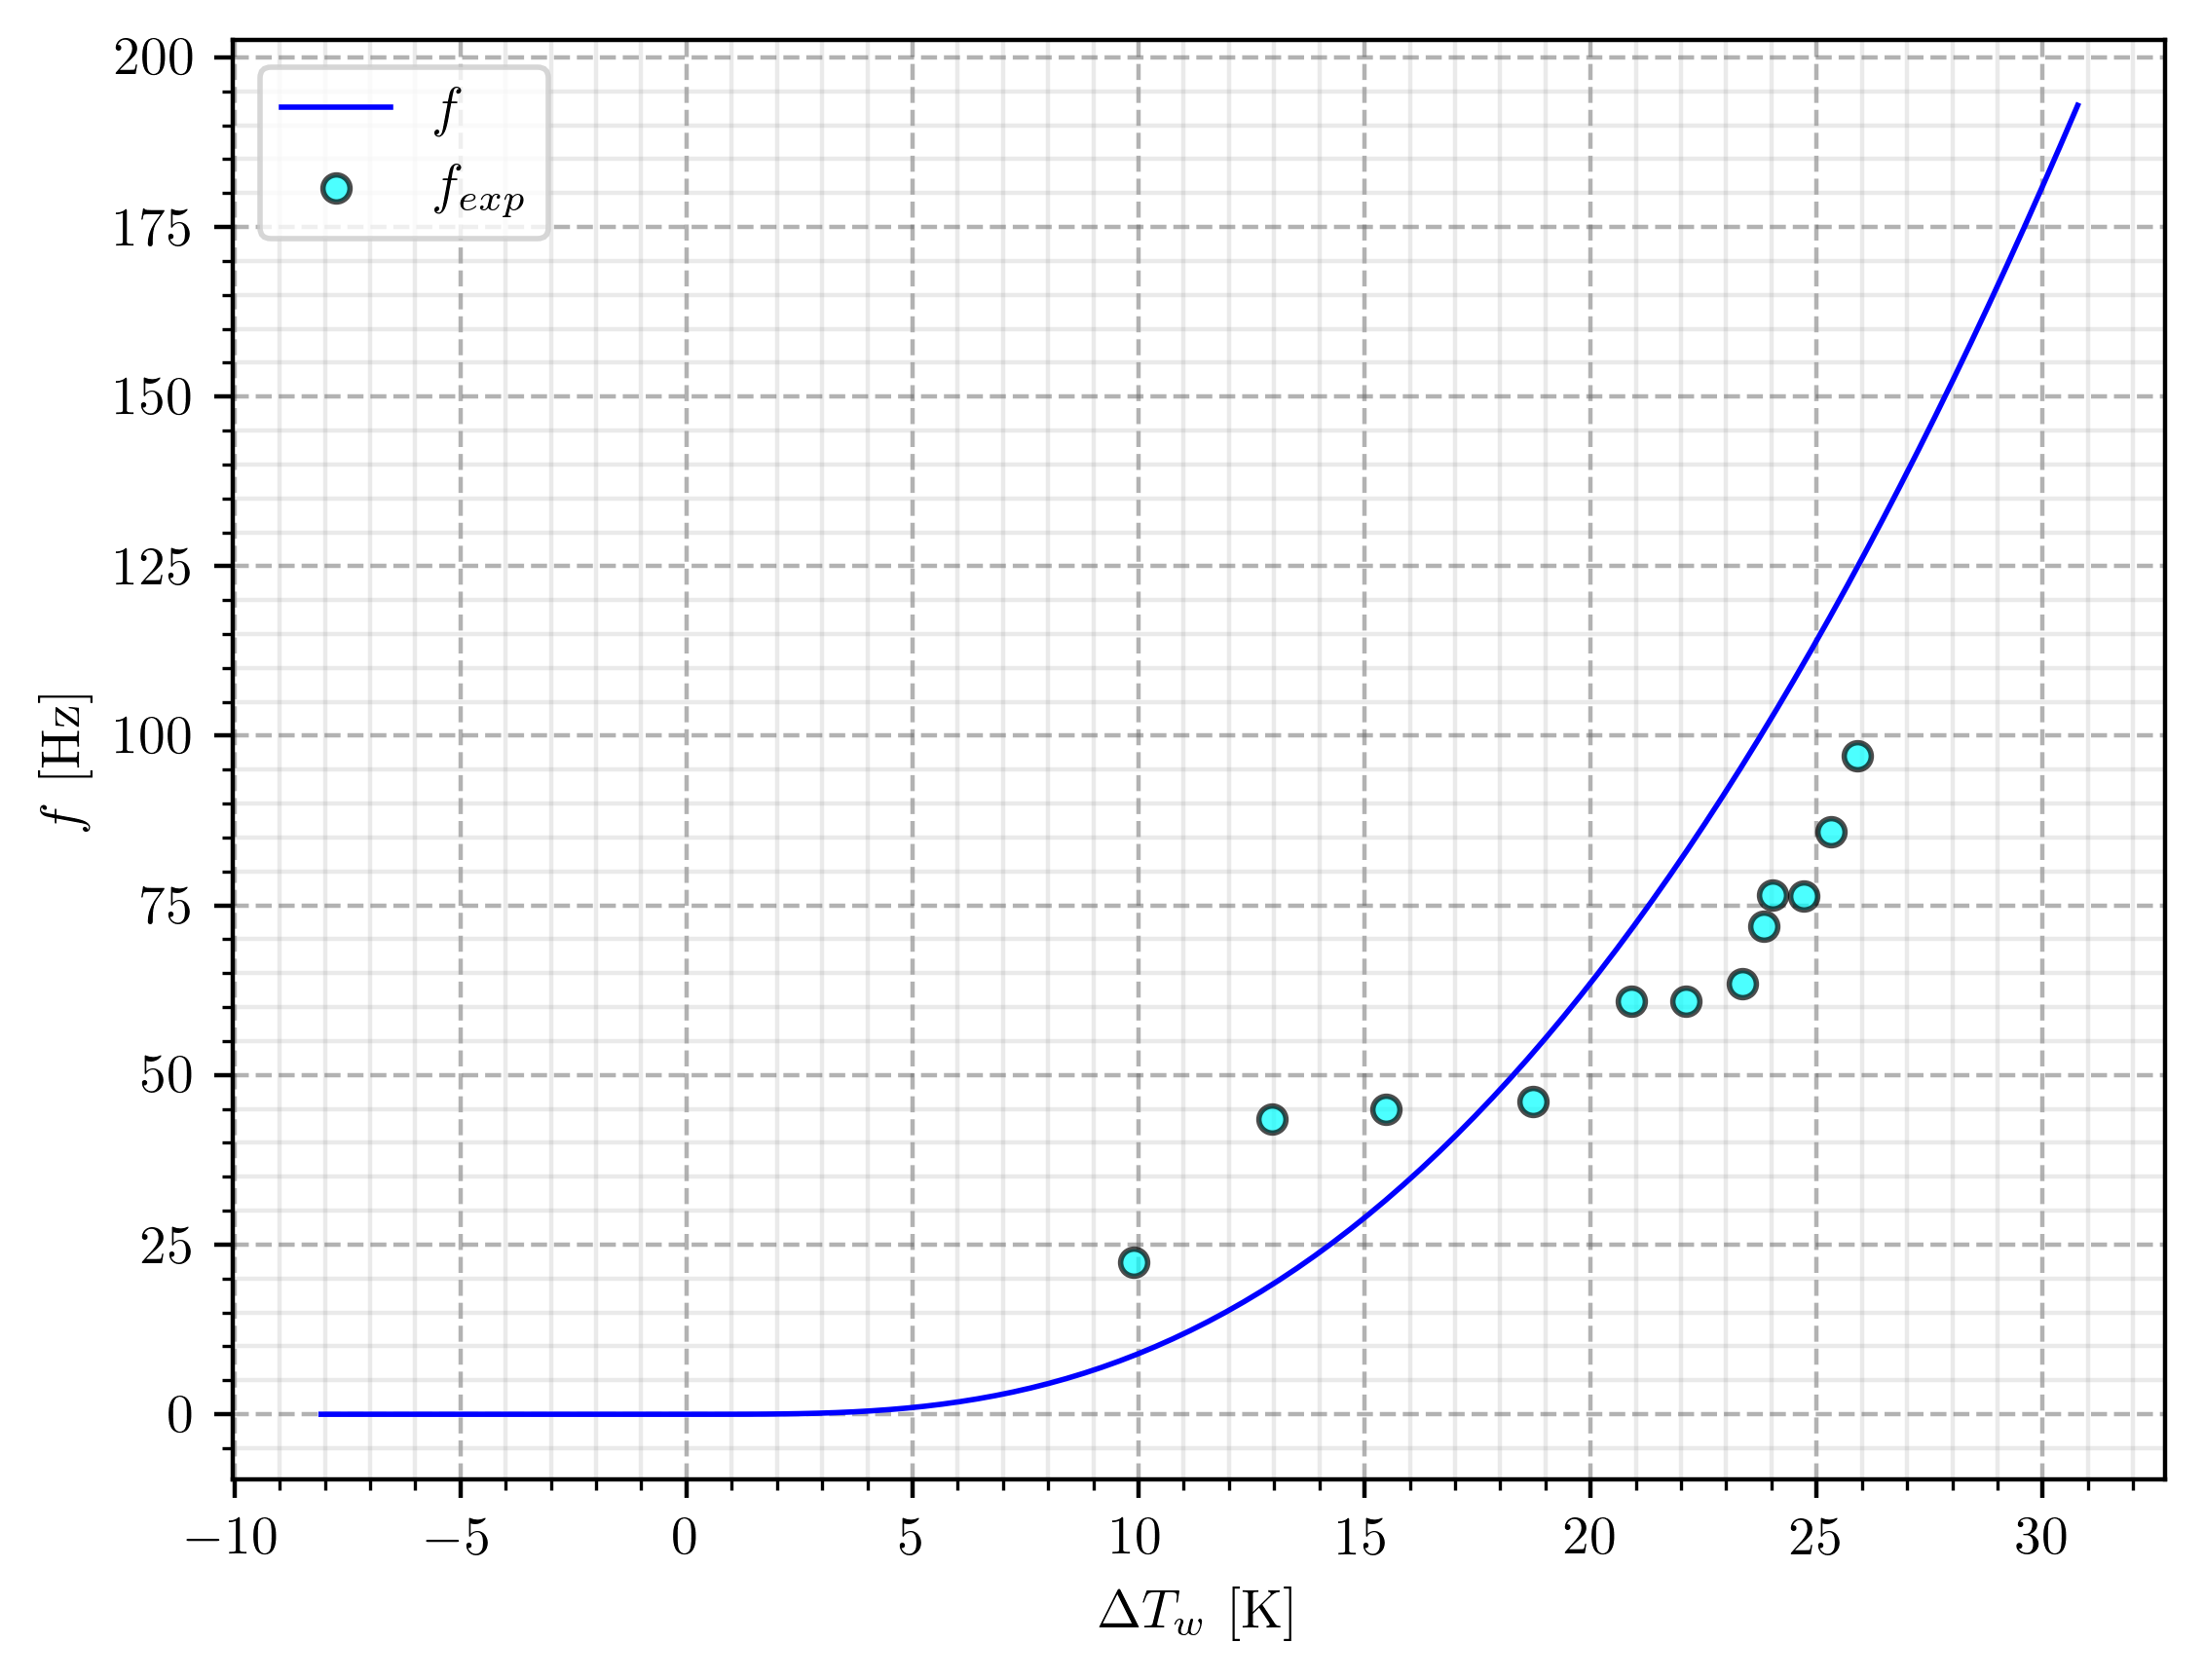
\includegraphics[width=0.5\linewidth]{img/HFP/fullcomp_Koss/f_G2000.png}
}
\subfloat[Bubble wait time, growth time and quenching time]{
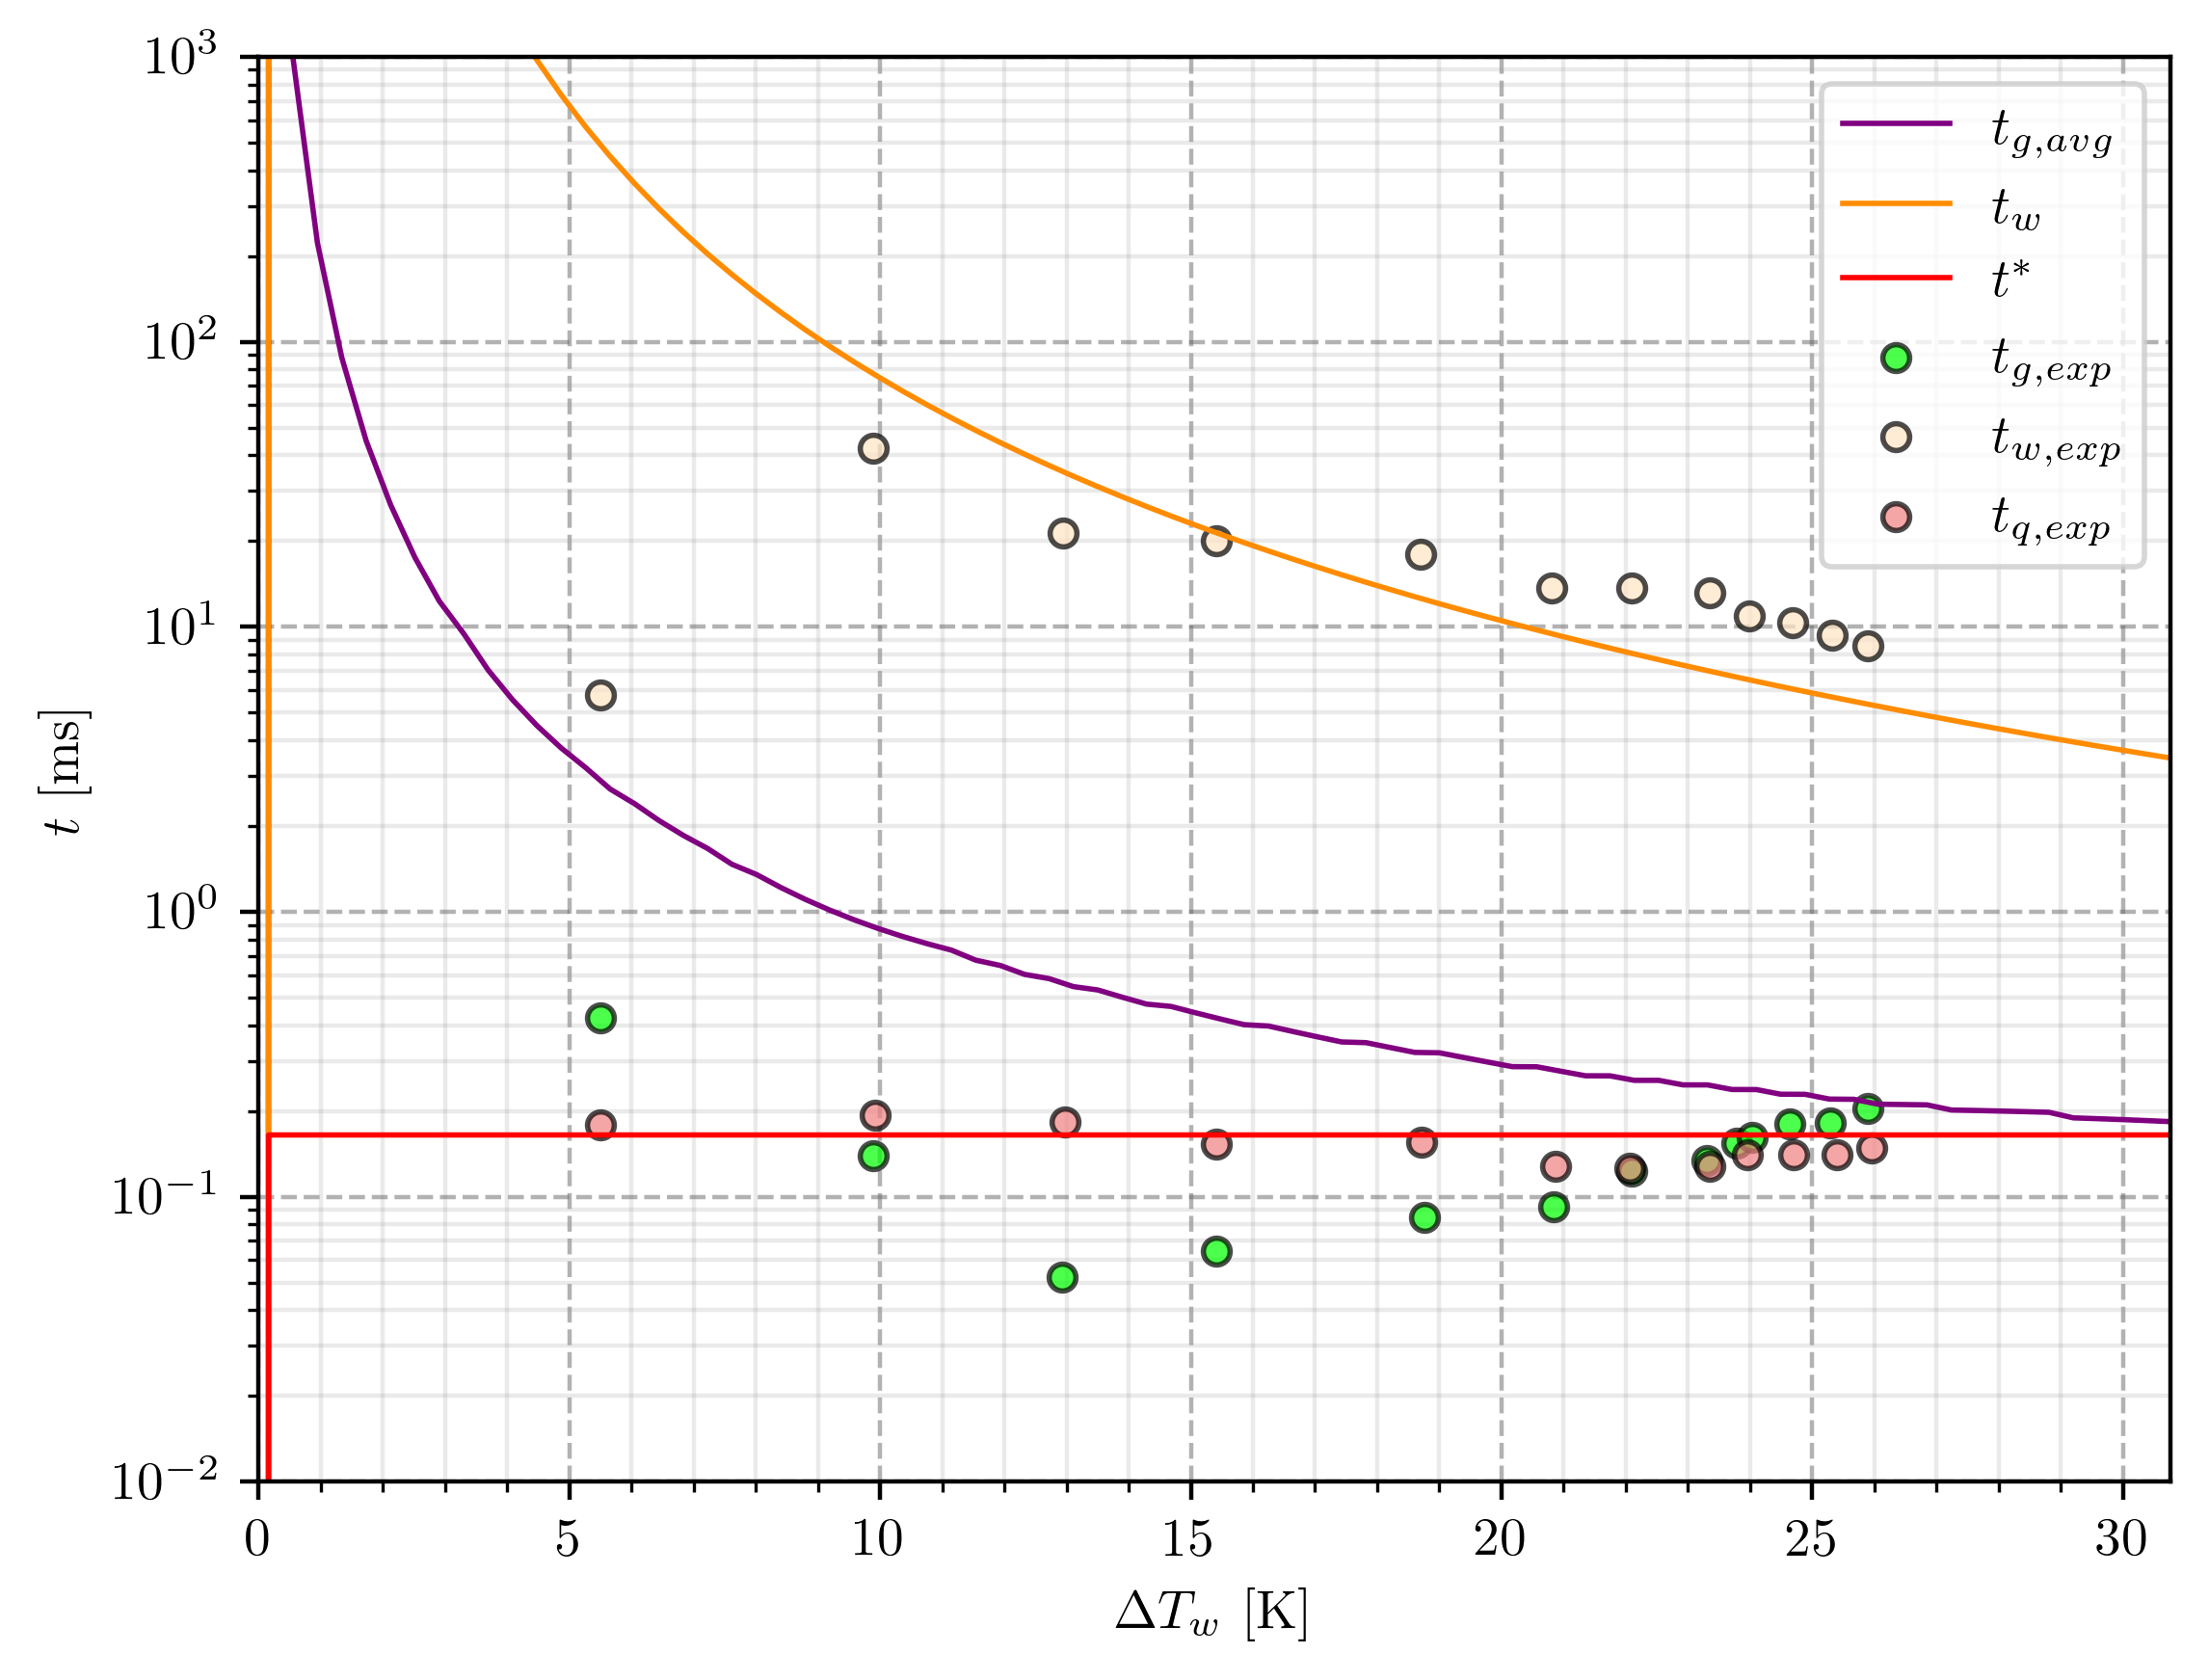
\includegraphics[width=0.5\linewidth]{img/HFP/fullcomp_Koss/times_G2000.png}
}
\caption{Comparison of bubble nucleation frequency, wait time, avergae growth time and quenching time.}
\label{fig:fullkoss_times}
\end{figure}


\subsection{Single Bubble Area and Total Bubble Area}

\begin{figure}[!h]
\subfloat[Single bubble area]{
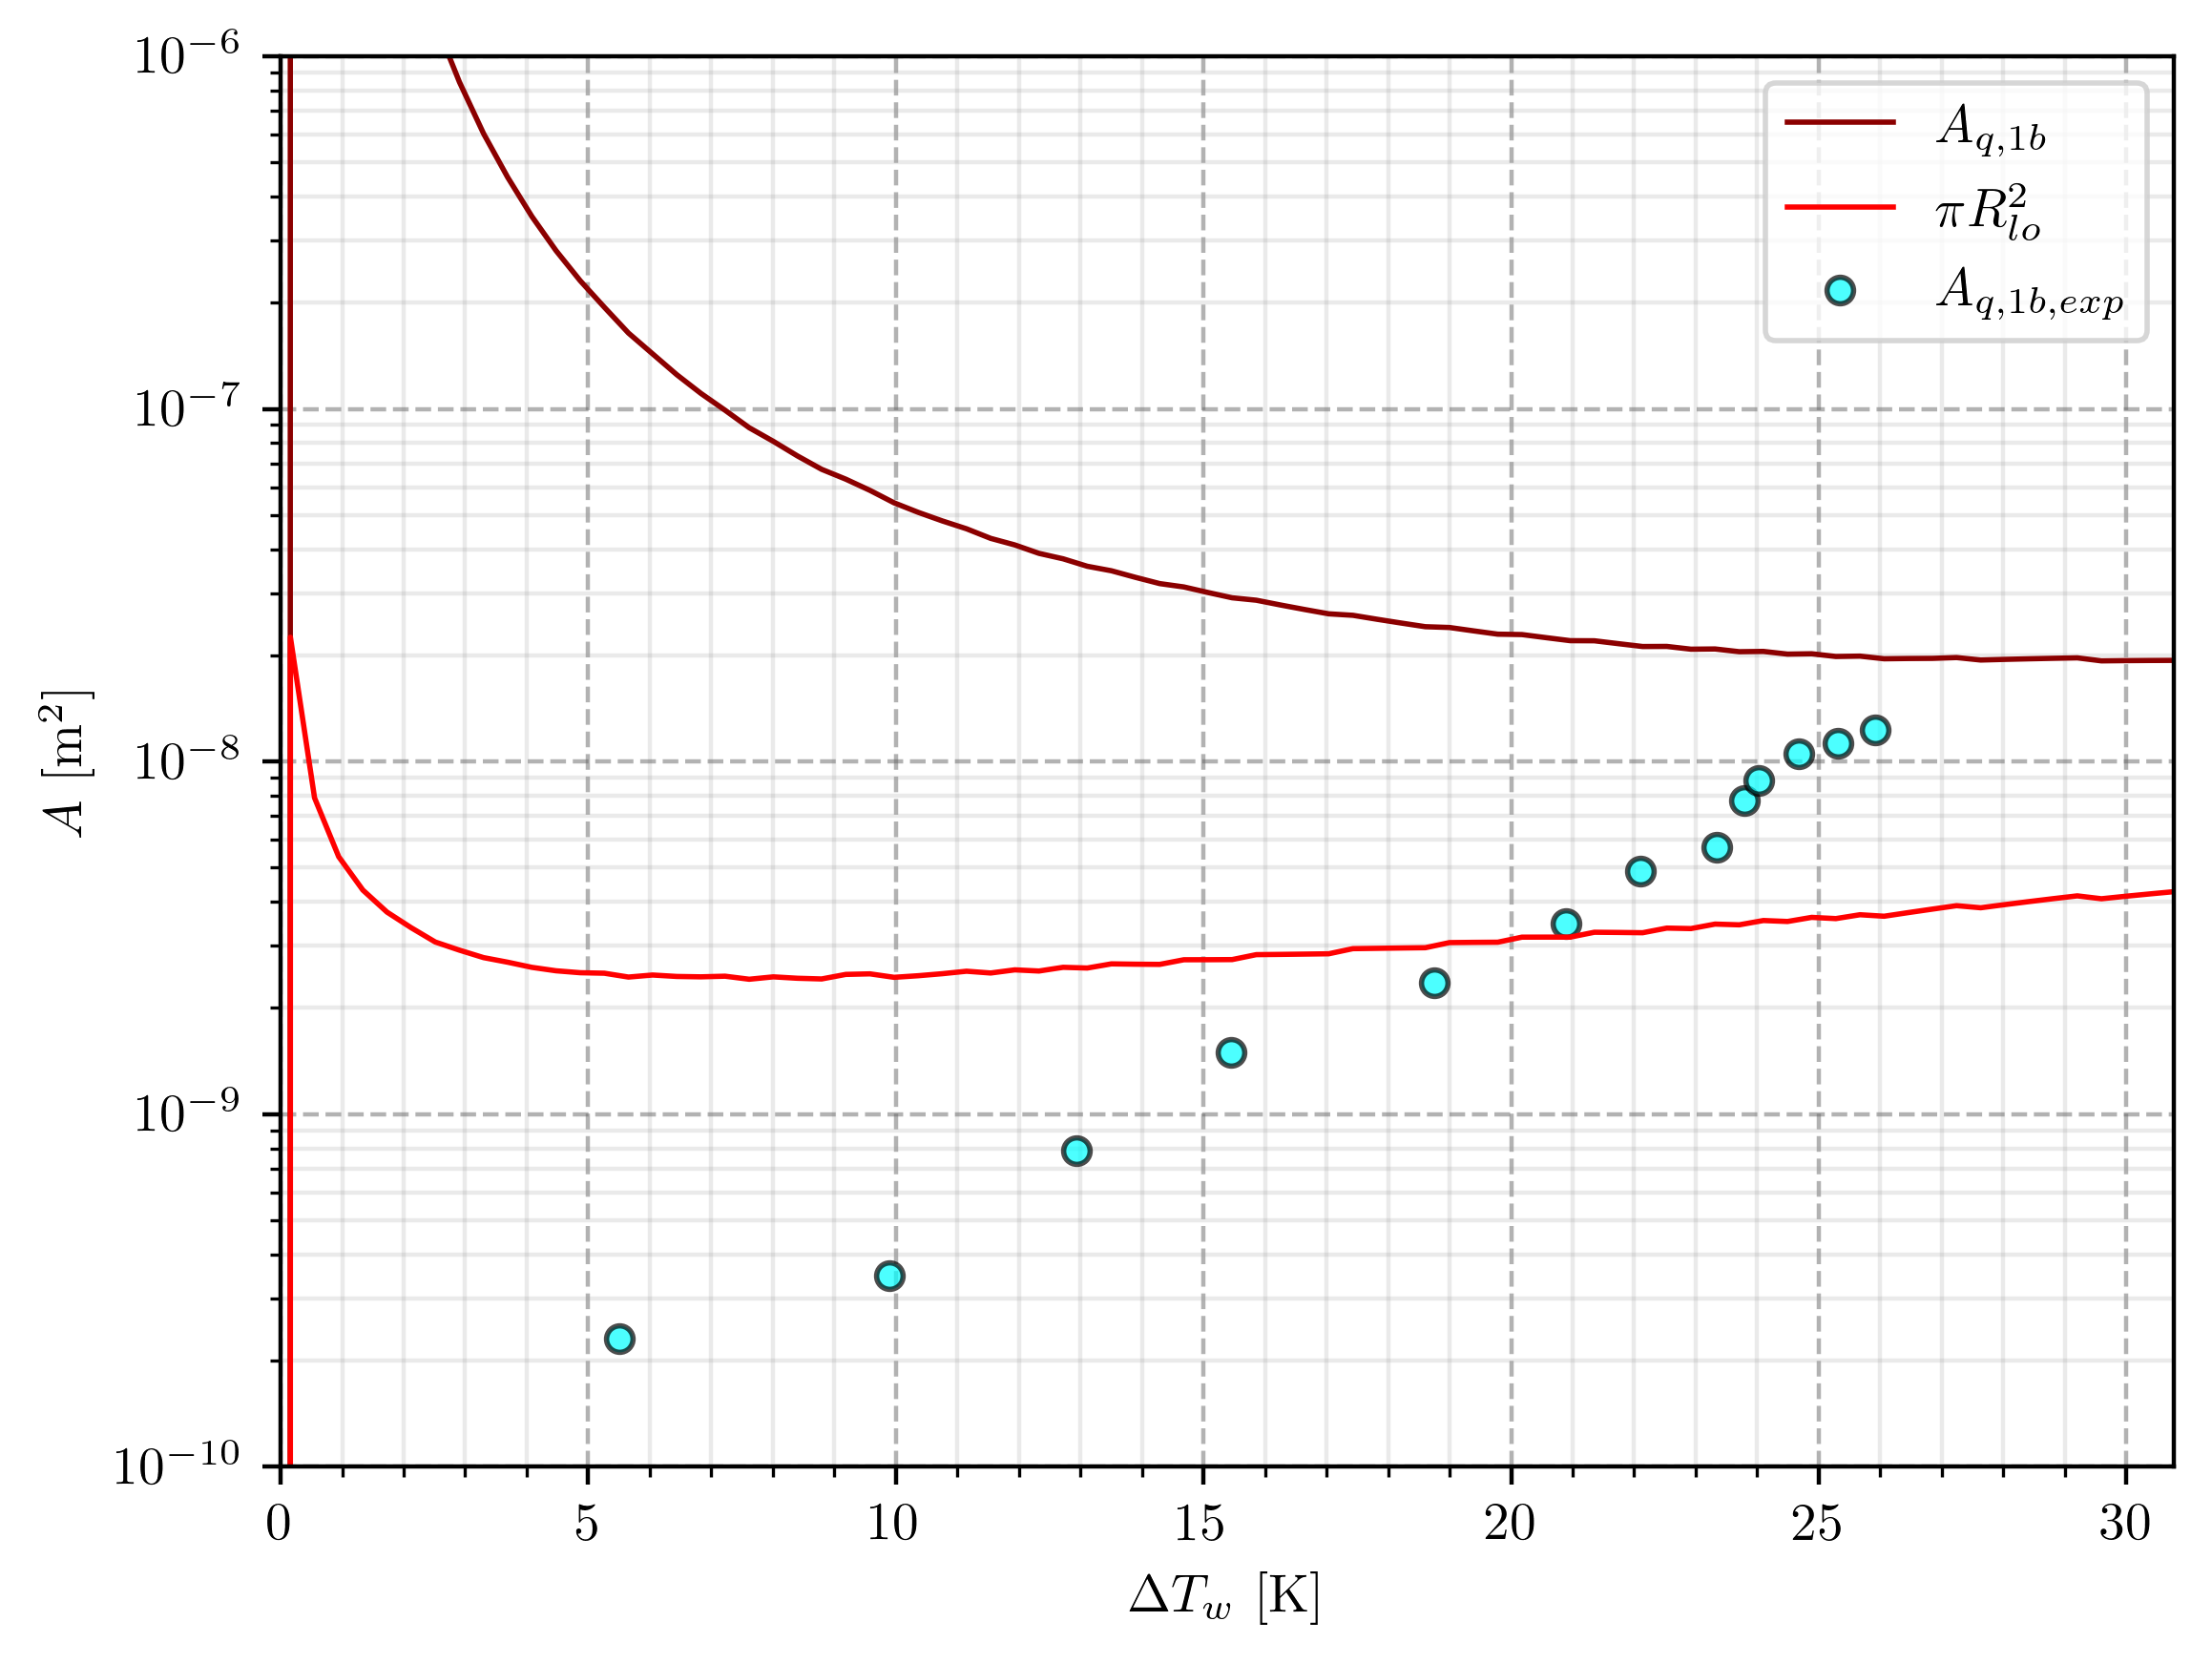
\includegraphics[width=0.5\linewidth]{img/HFP/fullcomp_Koss/Aq1b_G2000.png}
}
\subfloat[Total wall area impacted by bubbles]{
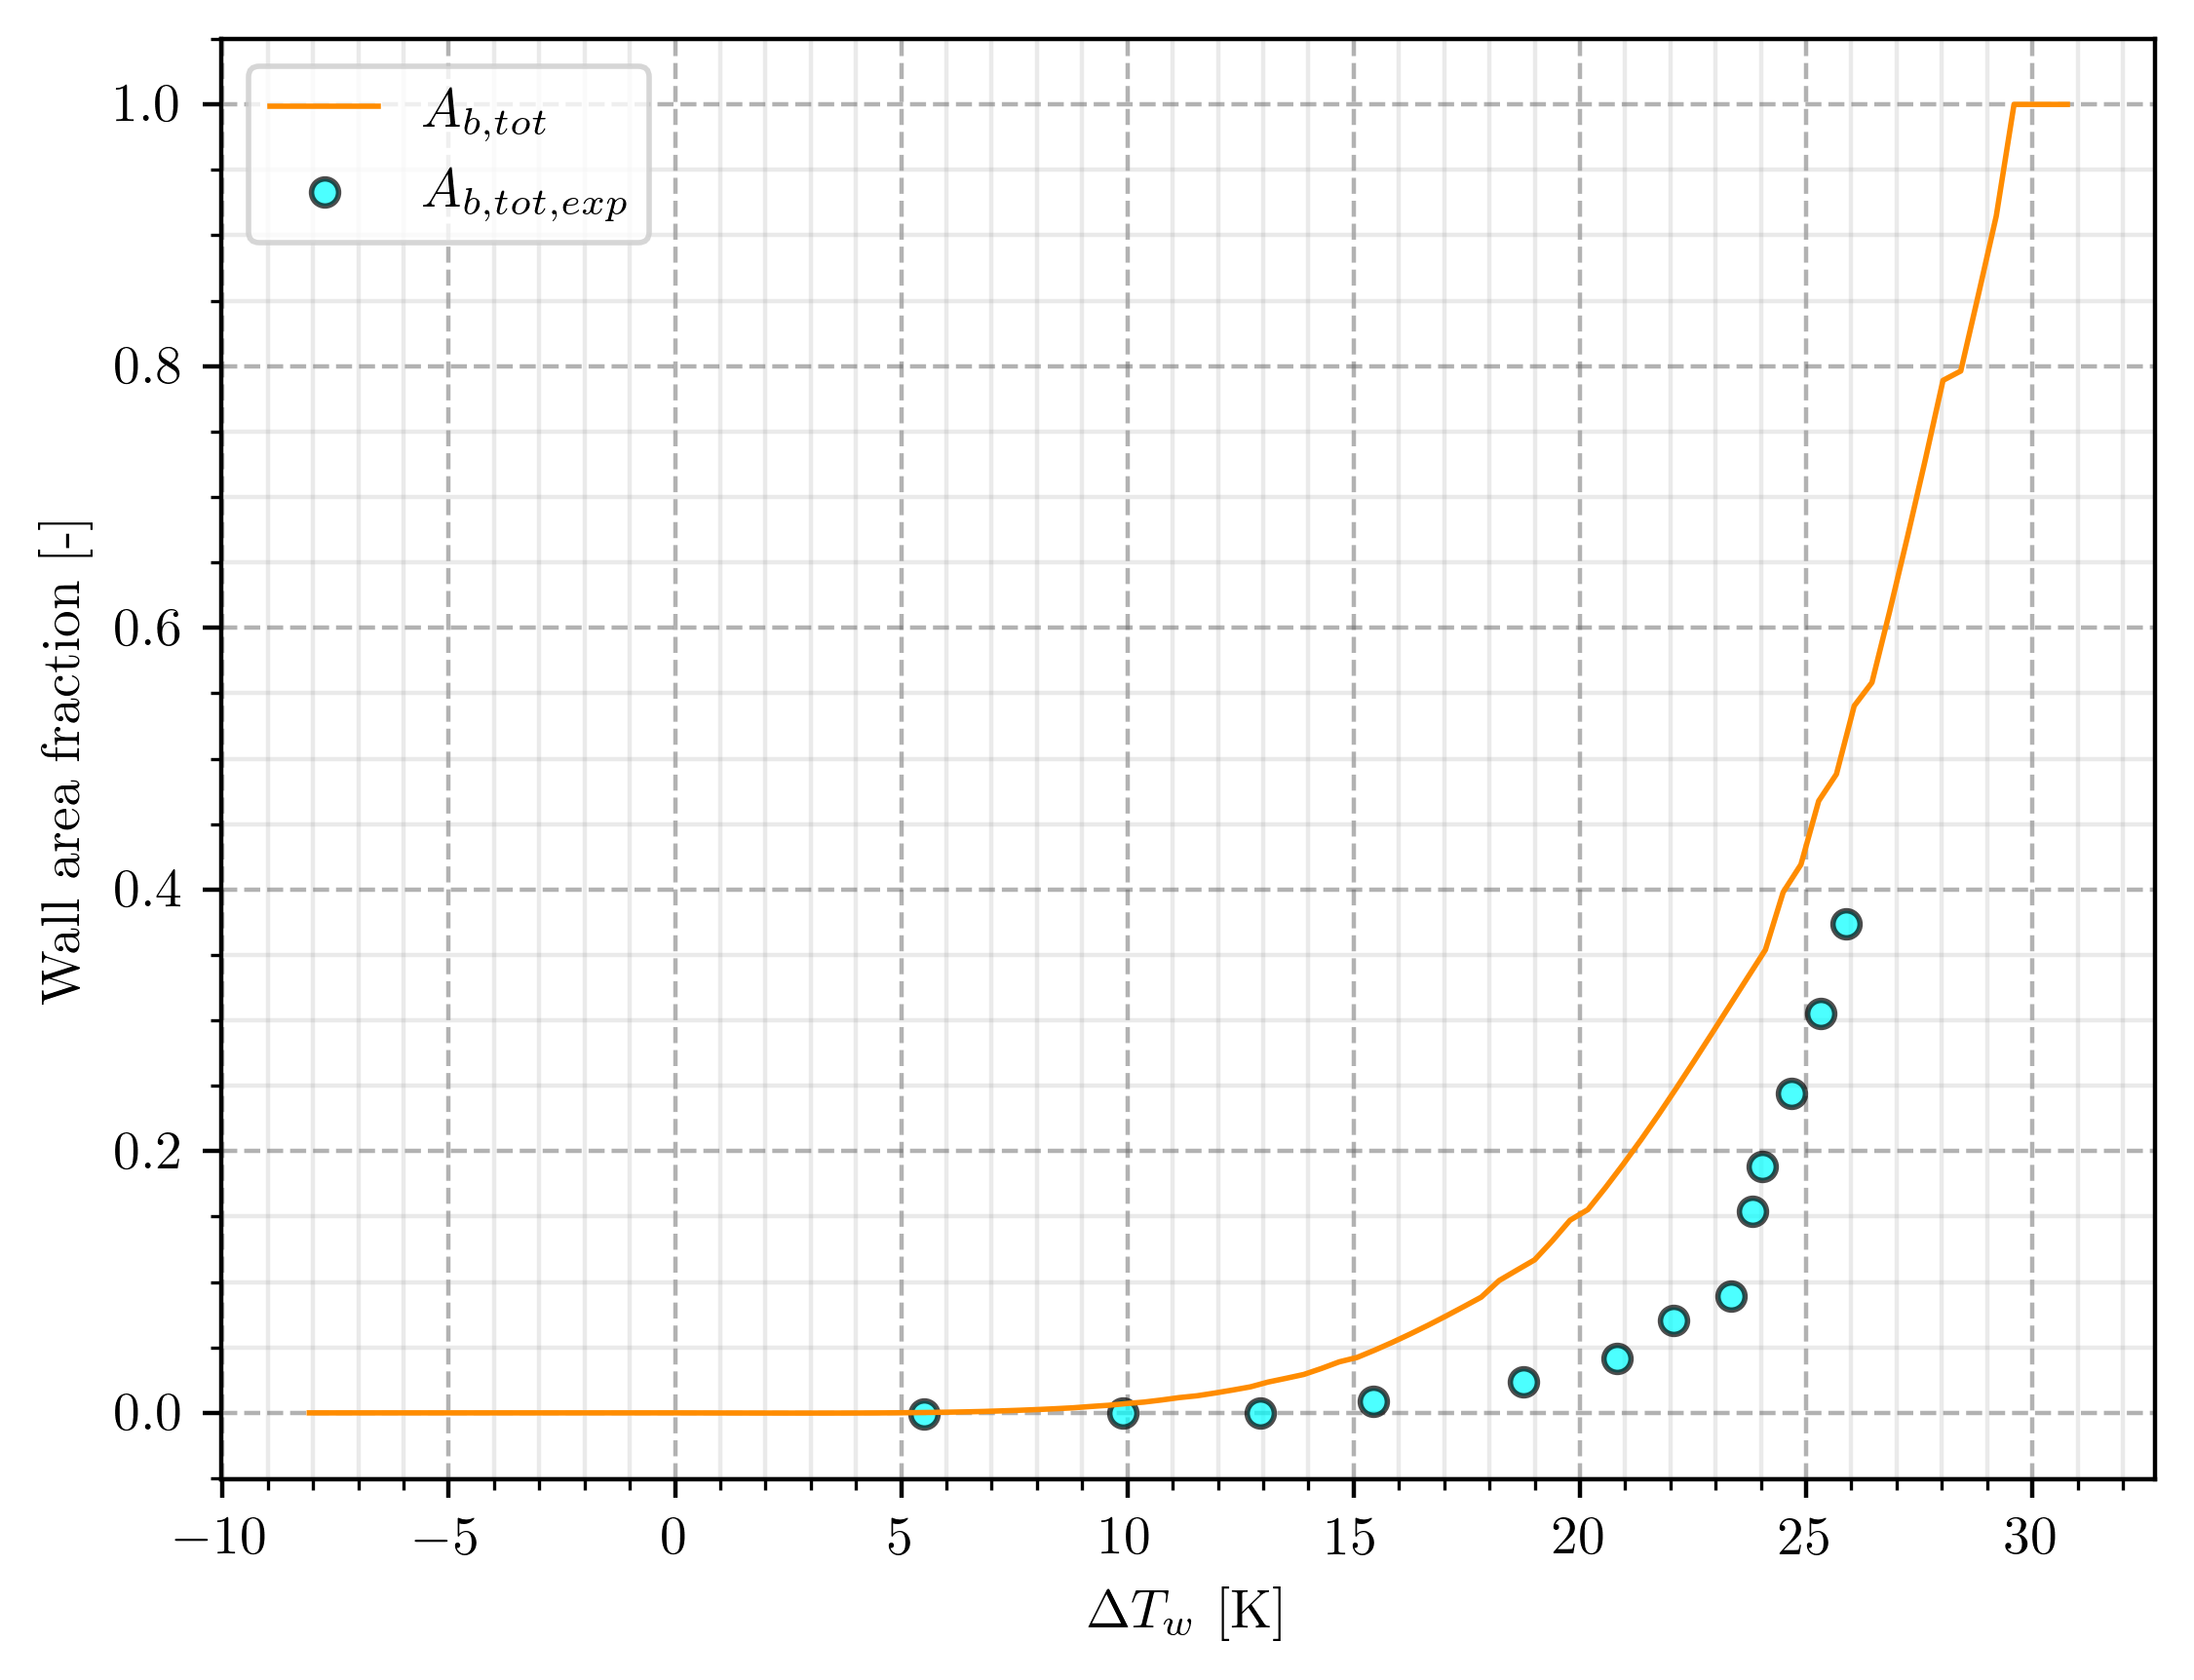
\includegraphics[width=0.5\linewidth]{img/HFP/fullcomp_Koss/Abub_tot_G2000.png}
}
\end{figure}


\begin{figure}[!h]
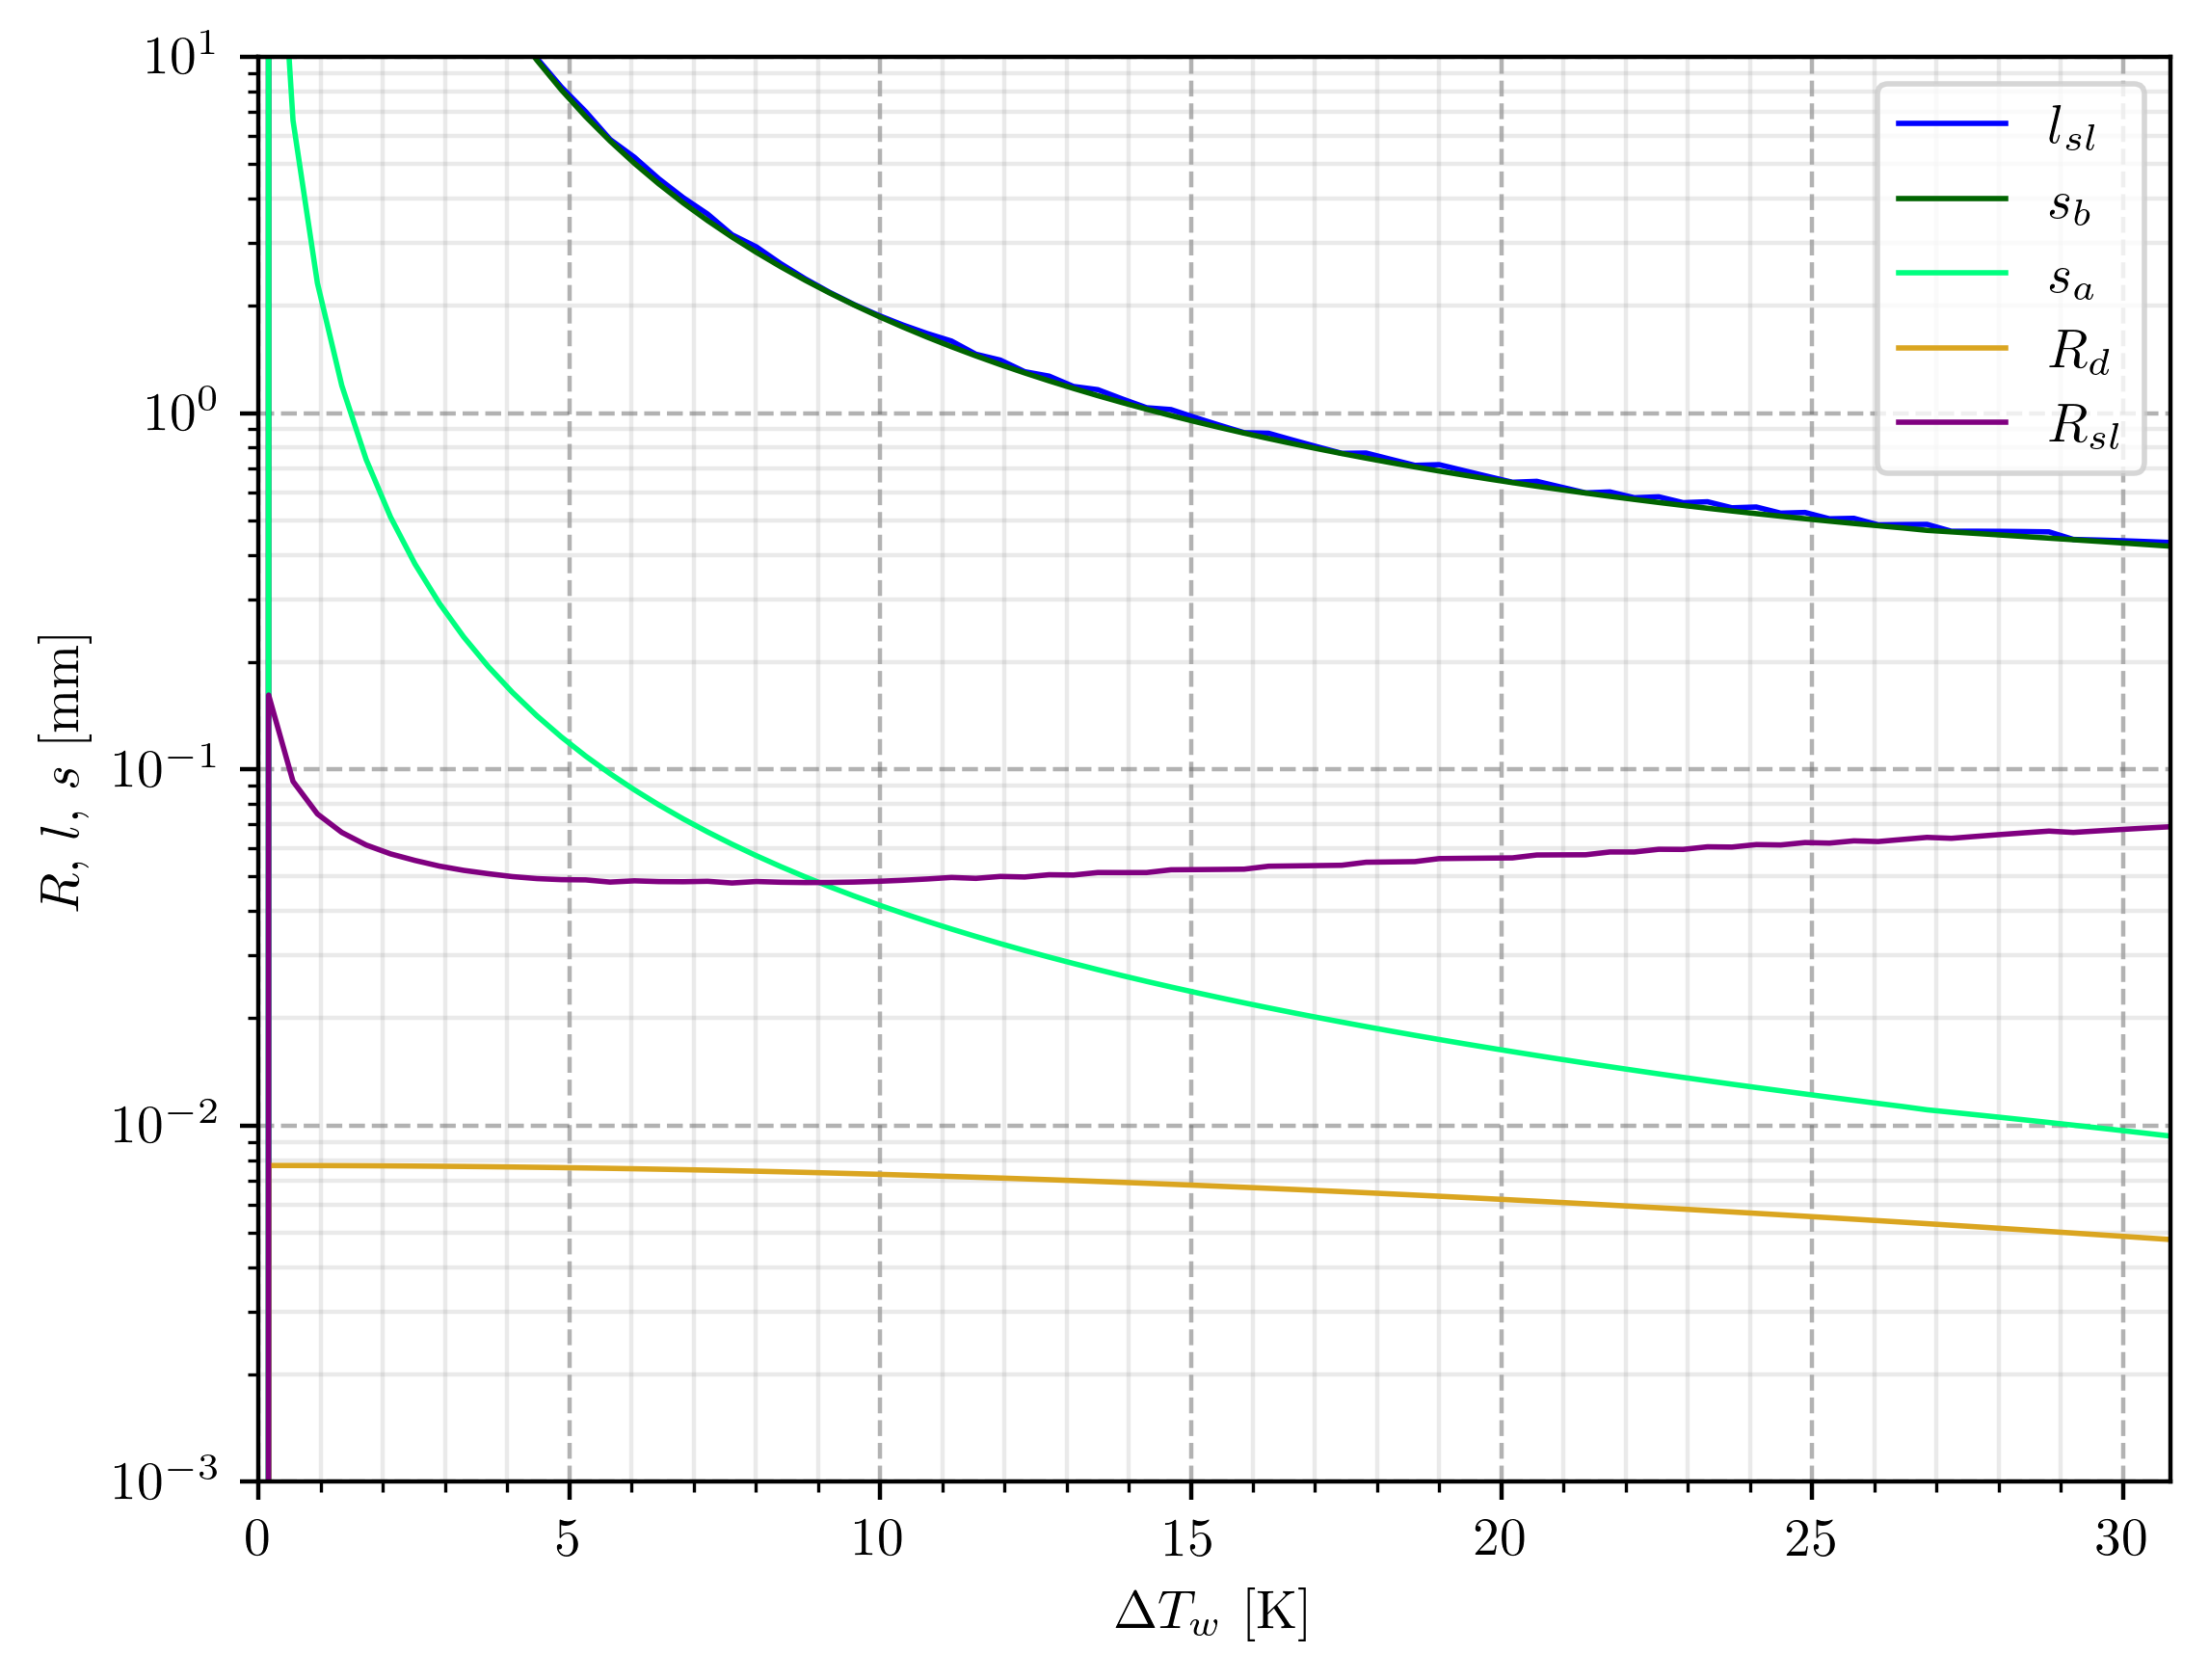
\includegraphics[width=0.5\linewidth]{img/HFP/fullcomp_Koss/length_G2000.png}
\end{figure}

\subsection{Flux Proportions and Wall Superheat}

\begin{figure}[!h]
\subfloat[Single bubble area]{
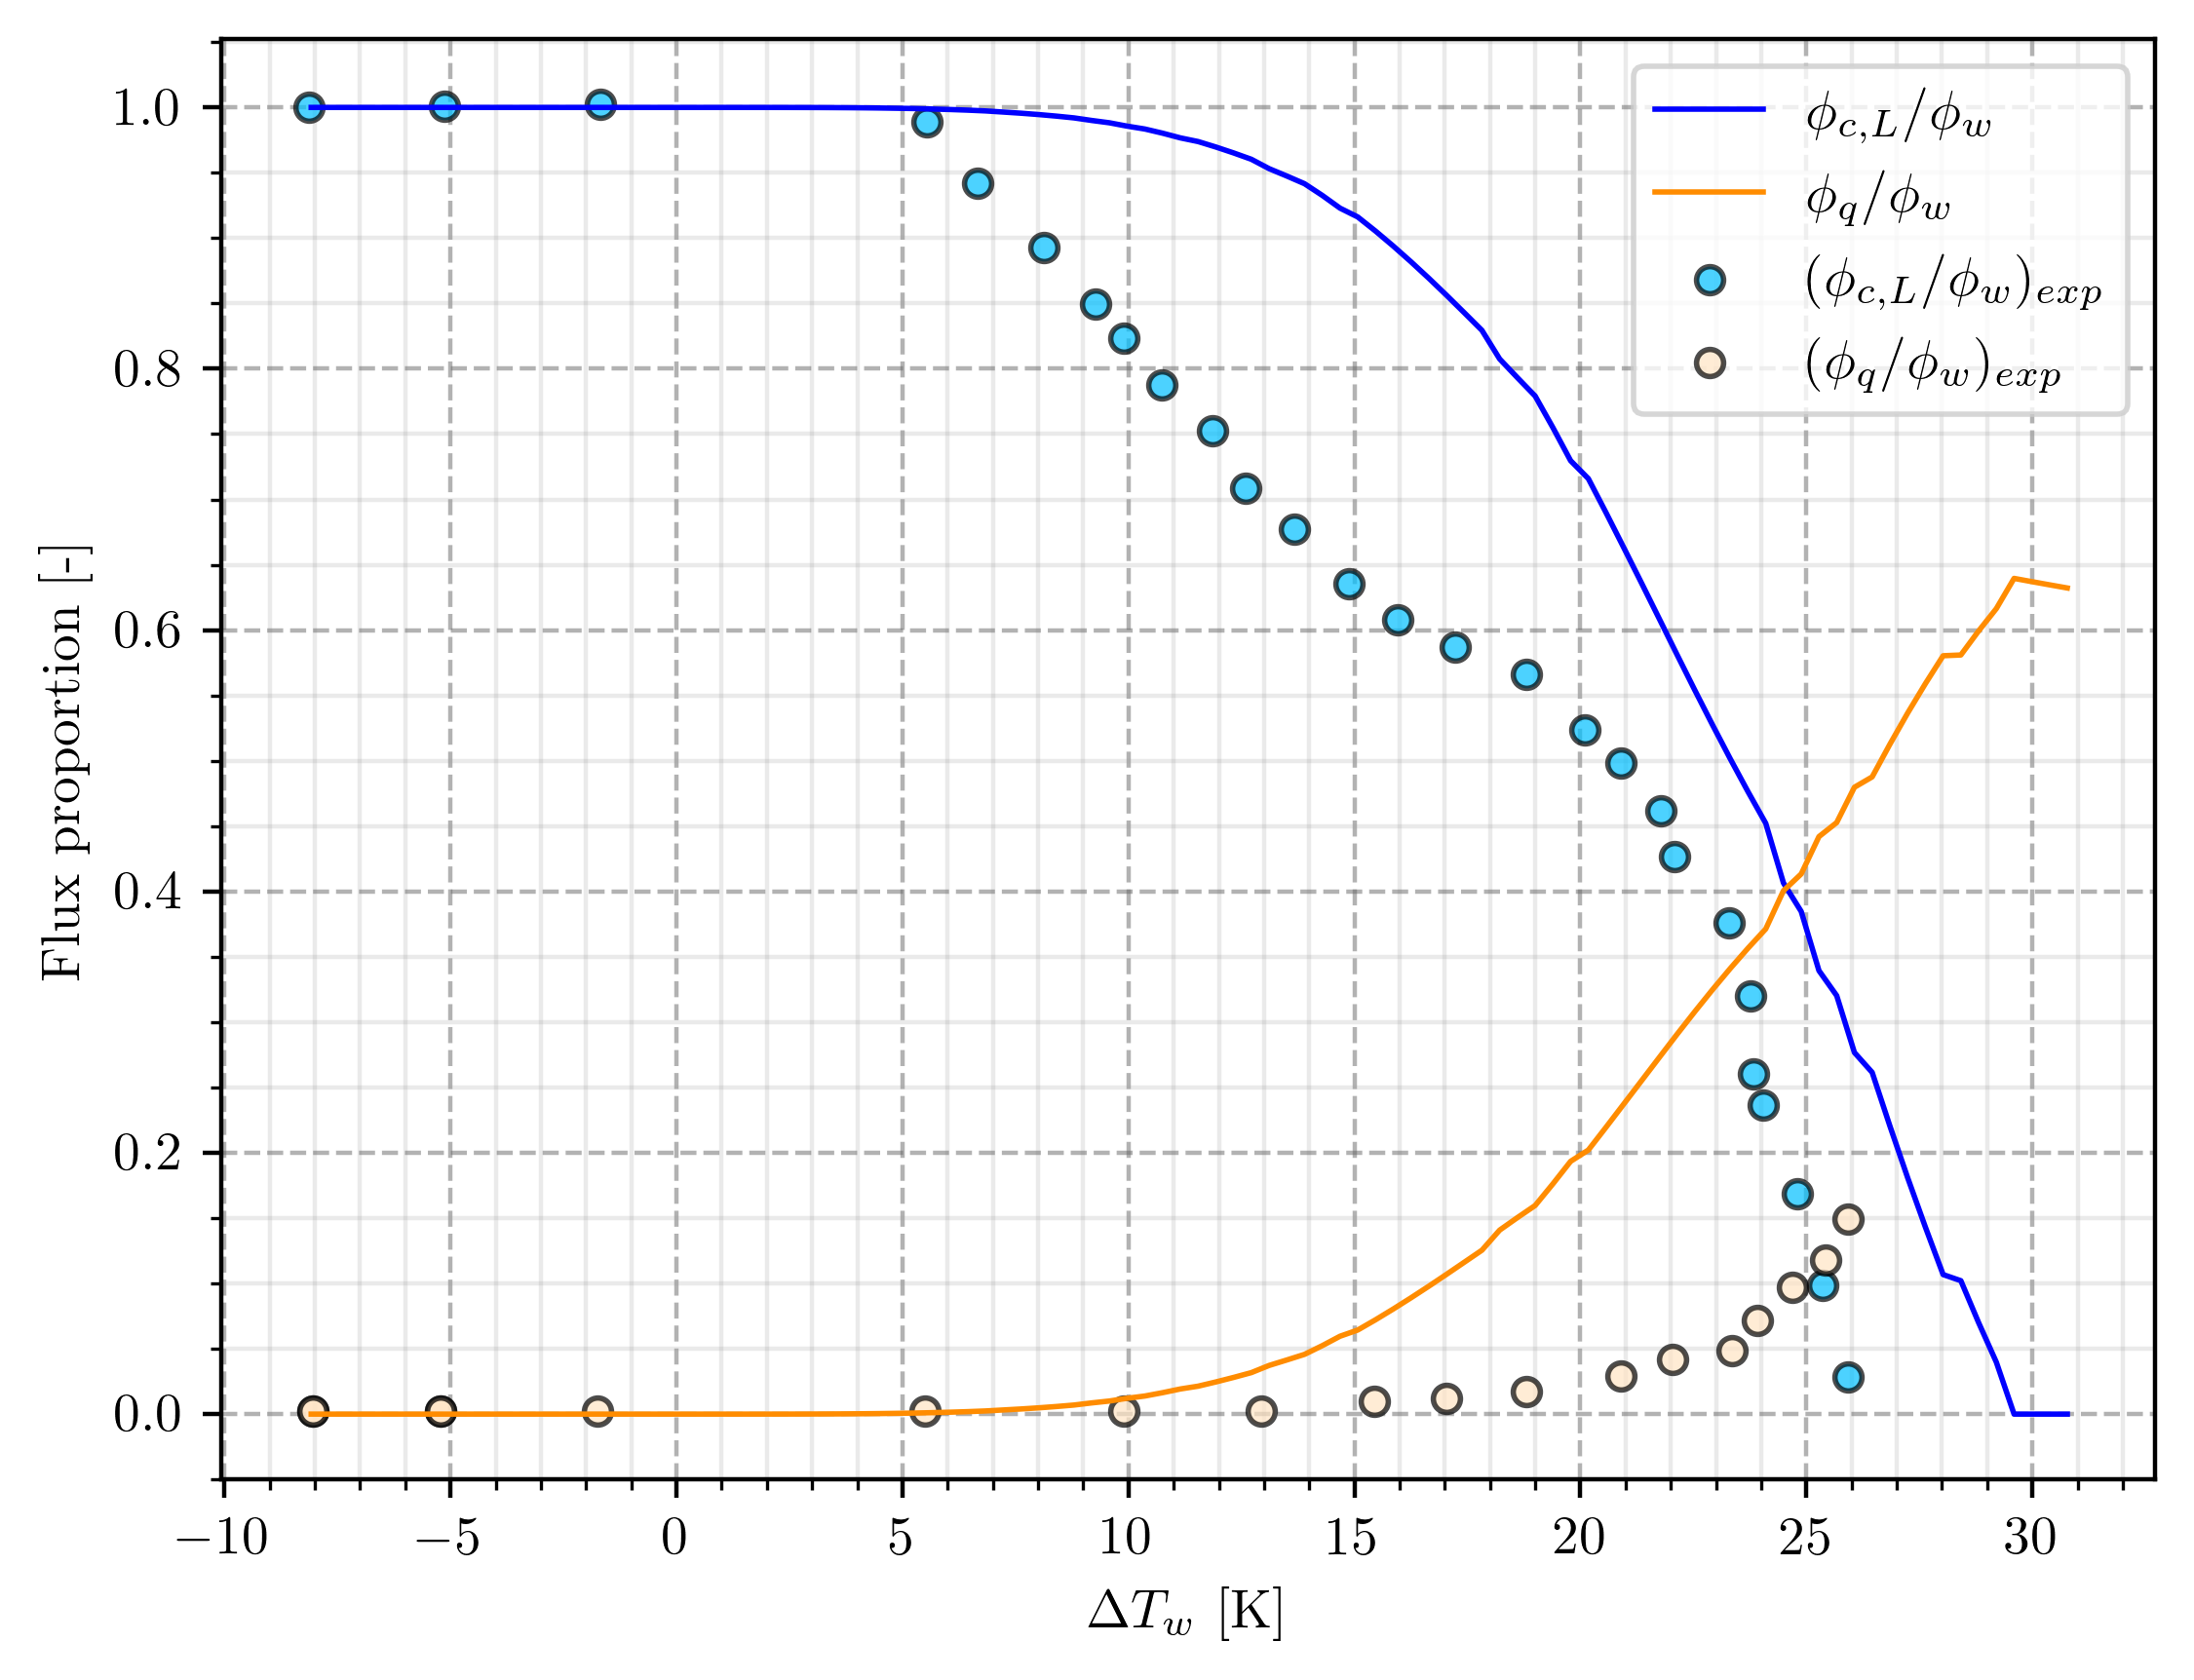
\includegraphics[width=0.5\linewidth]{img/HFP/fullcomp_Koss/hfp_G2000.png}
}
\subfloat[Total wall area impacted by bubbles]{
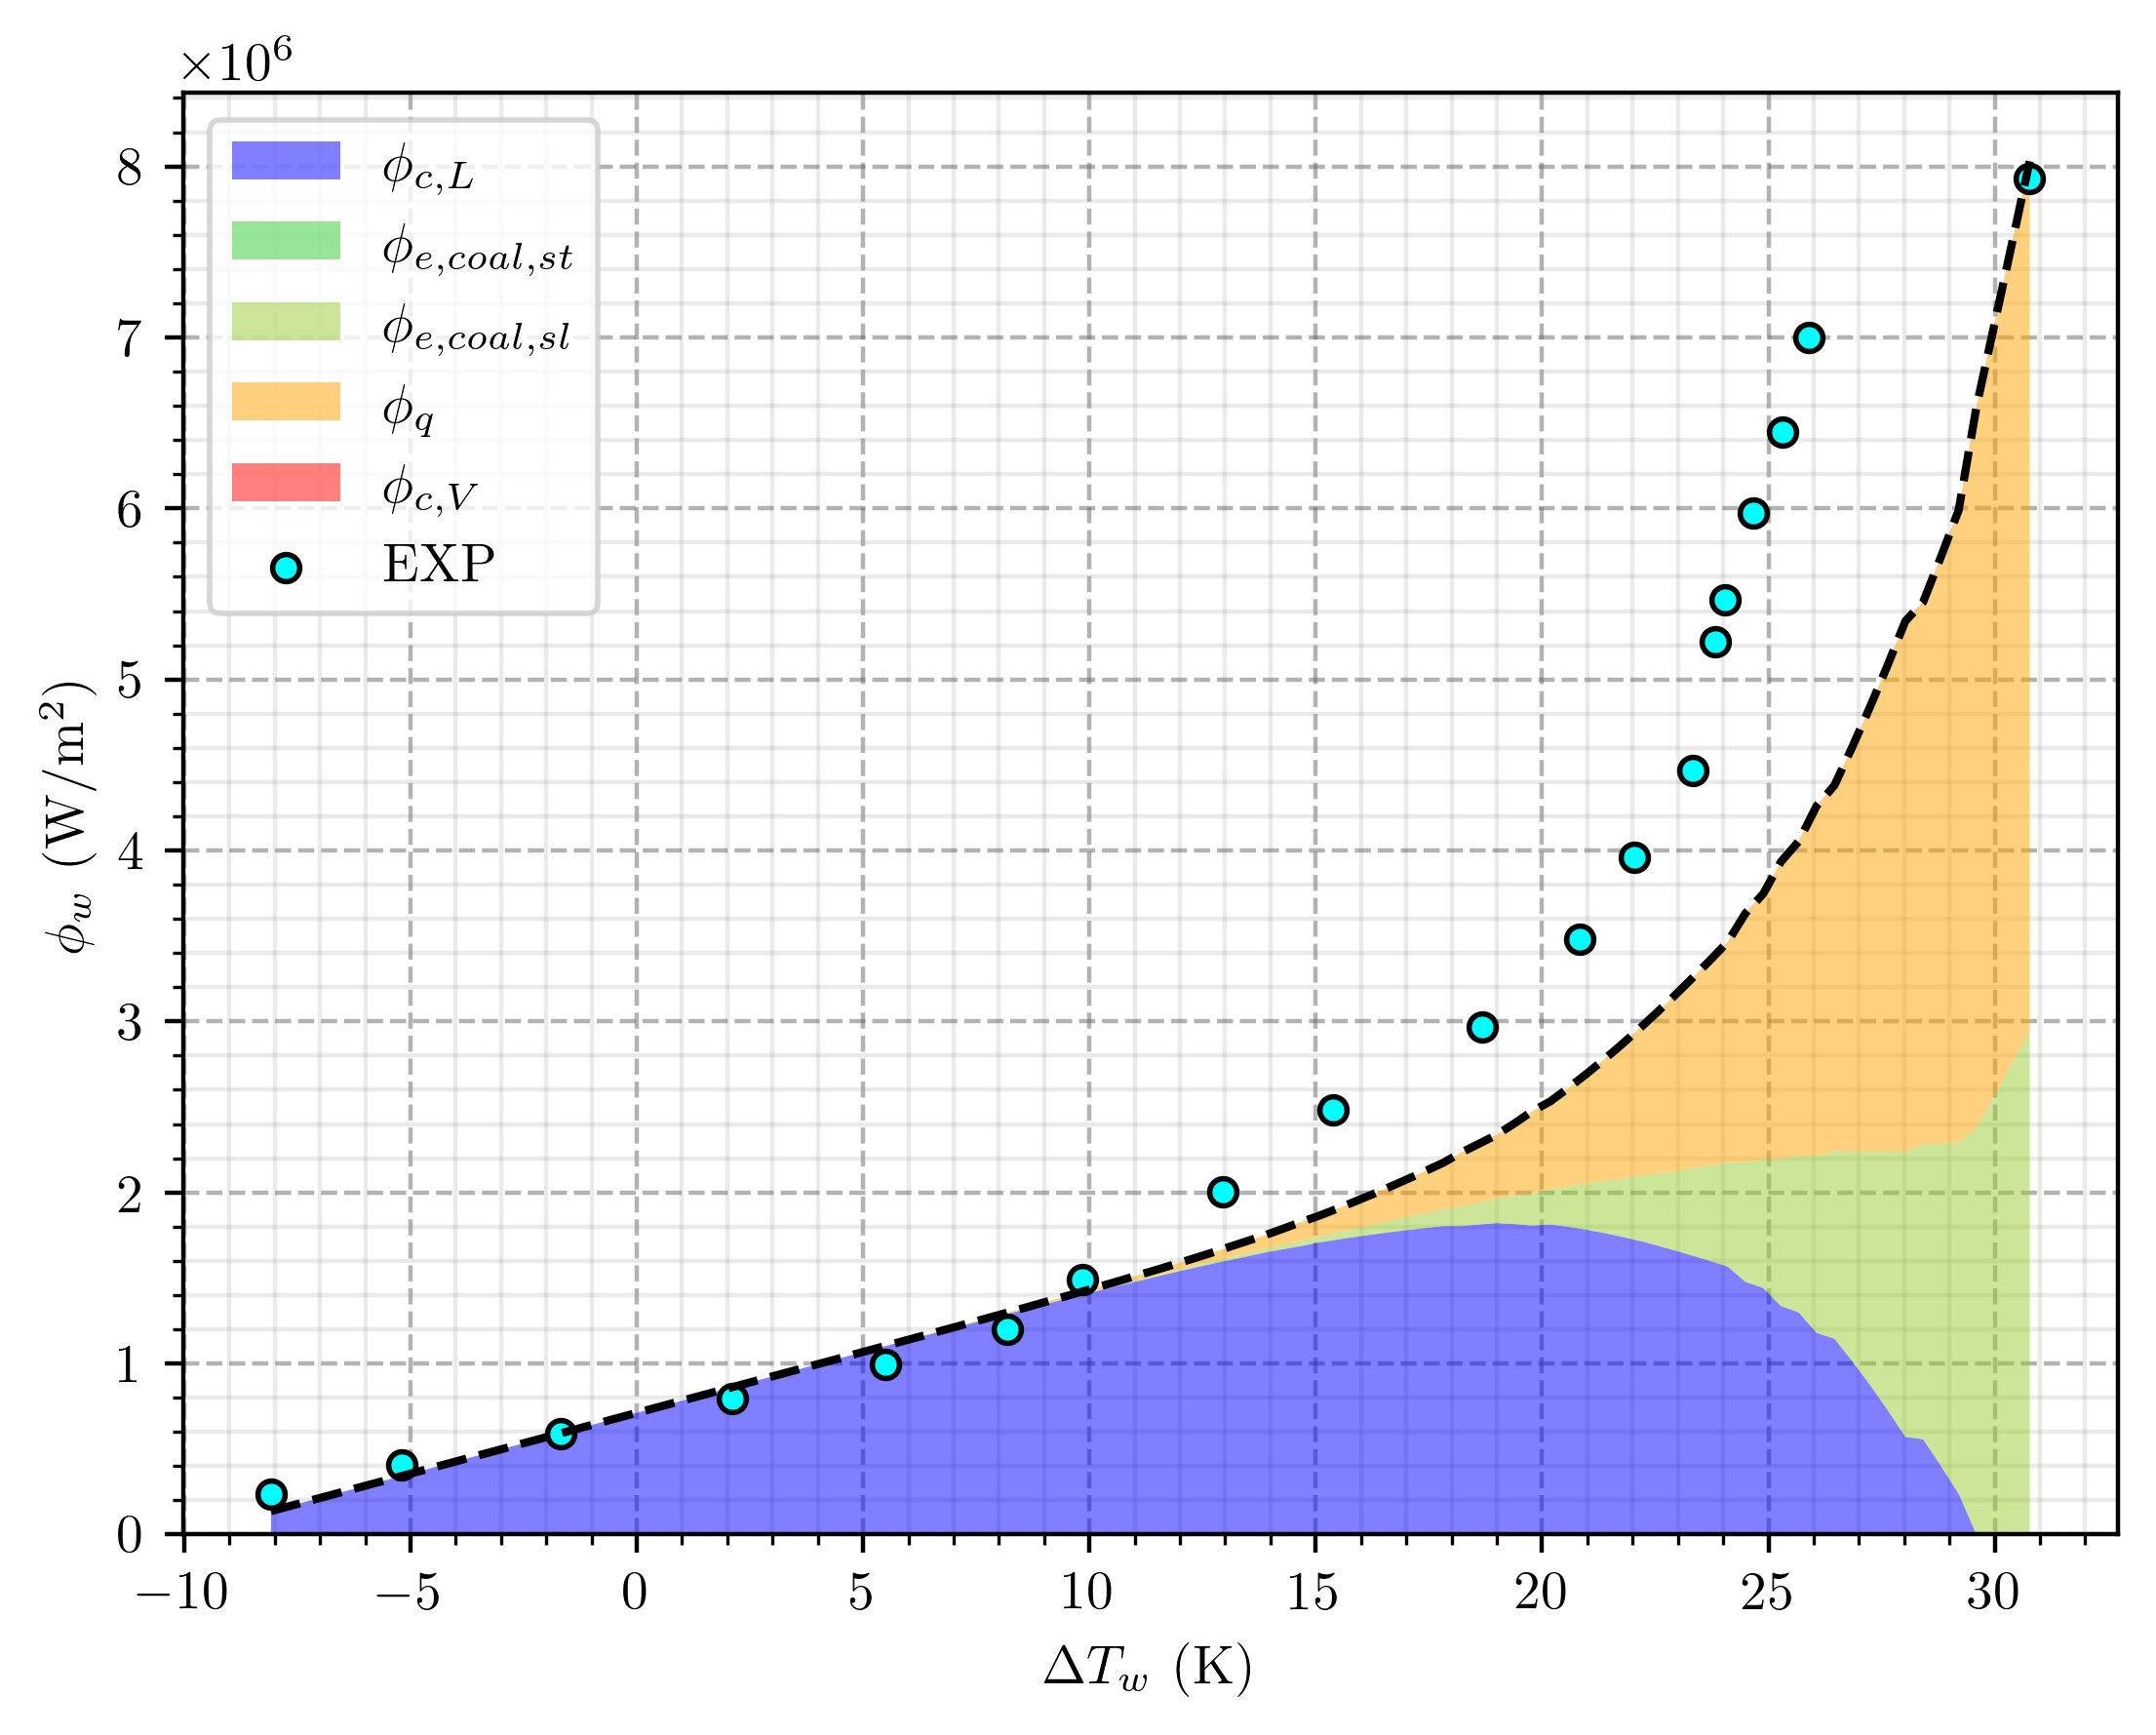
\includegraphics[width=0.5\linewidth]{img/HFP/fullcomp_Koss/boil_curve_G2000.png}
}
\end{figure}




\section{Wall Temperature Predictions}





\begin{table}[h!]

%\begin{changemargin}{-1cm}{0cm}

\noindent\makebox[\textwidth]{

\scriptsize
\centering
\begin{tabular}{p{20mm}|c c c c c c c c} 
Author & $D_{h}$ [mm] & $P$ [bar] & $G_{L}$ [$\debm$] & $\Delta T_{L}$ [K] & $\phi_{w}$ [MW/m\up{2}] & $T_{sat}-T_{w}$ [K] &$N_{mes}$ [-] \\
\hline
\\

Kossolapov \cite{kossolapov_experimental_2021} \newline (2021) & 12 & 1.12 - 75.8 & 500 - 2000 & 10 & 0.1 - 0.6  & 0.22 - 9.5 & 12 \\

Richenderfer \cite{richenderfer_experimental_2018} \newline (2018) & 15 & 1 - 5 & 1000 - 2000 & 10-20 & 0.1 - 0.63 & 1 - 18.7 & 13 \\

Jens-Lottes \cite{jens_analysis_1951} \newline (1951) & 5.74 & 137.9 & 2617.5 & 53.3 - 92.2 & 0.91 - 2.37 & 0.33 - 44.1 & 15 \\

Kennel \cite{kennel_local_1949} \newline (1948) & 4.3 - 13.2 & 2 - 6.2 & 284 - 10~577 & 11.1 - 83.3 & 0.035 - 1.89 & 0.35 - 69 & 52 \\
\hline
\end{tabular}
}
\caption{Experimental data range of wall temperature measurements from the single-phase part of boiling curves.}
\label{tab:exp_data_convection}
\end{table}
